\documentclass[10pt]{article}

\usepackage[T1]{fontenc}
\usepackage{geometry}
\usepackage{amsmath, amssymb, amsthm}
\usepackage{tikz}

\geometry{a4paper, margin=1in}
\setlength\parindent{0pt}
\renewcommand{\labelenumi}{(\roman{enumi})}
% \renewcommand\qedsymbol{$\blacksquare$}

\renewcommand{\land}{\text{ and }}
\renewcommand{\lor}{\text{ or }}
\newcommand{\compl}{\mathsf{c}}

\newcommand\blfootnote[1]{%
    \begingroup
    \renewcommand\thefootnote{}\footnote{#1}%
    \addtocounter{footnote}{-1}%
    \endgroup
}


\title{
    \textsc{
        \large
        MA1101: Mathematics I
    }
    \\\vspace{0.2em}
    \textbf{
        \huge
        Solutions for Problem Sheet II
    }
    \vspace{-1em}
}
\author{}
\date{}

\begin{document}

    \maketitle
    \blfootnote{
        Satvik Saha (\texttt{ss19ms154@iiserkol.ac.in})
    }



    \paragraph{Problem 1.}
    Denote $X = \{1, 2, 3, 4, 5\}$ and $\Delta = \{(1, 1), (2, 2), (3, 3), (4,
    4), (5, 5)\}$, i.e.\ the \emph{diagonal} of $X\times X$.
    We list examples of the described relations on $X$ without proof below.

    \begin{enumerate}
        \item Relations that are reflexive, not symmetric, not transitive.
        \begin{align*}
            R_{11} &= \Delta \cup \{(1, 2), (2, 3)\}, \\
            R_{12} &= \Delta \cup \{(2, 3), (3, 4)\}, \\
            R_{12} &= \Delta \cup \{(3, 4), (4, 5)\}.
        \end{align*}

        \item Relations that are not reflexive, are symmetric, not transitive.
        \begin{align*}
            R_{21} &= \{(1, 2), (2, 1)\}, \\
            R_{22} &= \{(2, 3), (3, 2)\}, \\
            R_{22} &= \{(3, 4), (4, 3)\}.
        \end{align*}

        \item Relations that are not reflexive, not symmetric, are transitive.
        \begin{align*}
            R_{31} &= \{(1, 2)\}, \\
            R_{32} &= \{(2, 3)\}, \\
            R_{32} &= \{(3, 4)\}.
        \end{align*}

        \item Relations that are reflexive, are symmetric, not transitive.
        \begin{align*}
            R_{41} &= \Delta \cup \{(1, 2), (2, 1), (2, 3), (3, 2)\}, \\
            R_{42} &= \Delta \cup \{(2, 3), (3, 2), (3, 4), (4, 3)\}, \\
            R_{42} &= \Delta \cup \{(3, 4), (4, 3), (4, 5), (5, 4)\}.
        \end{align*}

        \item Relations that are not reflexive, are symmetric, are transitive.
        \begin{align*}
            R_{51} &= \emptyset, \\
            R_{52} &= \{(1, 1)\}, \\
            R_{52} &= \{(2, 2)\}.
        \end{align*}

        \item Relations that are reflexive, not symmetric, are transitive.
        \begin{align*}
            R_{61} &= \Delta \cup \{(1, 2)\}, \\
            R_{62} &= \Delta \cup \{(2, 3)\}, \\
            R_{62} &= \Delta \cup \{(3, 4)\}.
        \end{align*}

        \item Relations that are not reflexive, not symmetric, not transitive.
        \begin{align*}
            R_{71} &= \{(1, 2), (2, 3)\}, \\
            R_{72} &= \{(2, 3), (3, 4)\}, \\
            R_{72} &= \{(3, 4), (4, 5)\}.
        \end{align*}

        \item Relations that are reflexive, are symmetric, are transitive.
        \begin{align*}
            R_{81} &= X\times X, \\
            R_{82} &= \Delta, \\
            R_{82} &= \Delta \cup \{(1, 2), (2, 1)\}.
        \end{align*}
    \end{enumerate}



    \paragraph{Problem 2.}
    Let $x \in X$ be arbitrary. Using the given property of $R$, there exists
    $a \in X$ such that $xRa$. By symmetry of $R$, we have $aRx$. Combining
    $xRa$ and $aRx$ using the transitivity of $R$, we have $xRx$.
    This proves that $R$ is reflexive. \qed


    \paragraph{Problem 3.}
    \begin{enumerate}
        \item For arbitrary $(x, y)\in\mathbb{R}^2$, we have $(x, y)\sim(x,
        y)$, since $x = x$. Therefore, $\sim$ is reflexive.

        Let $(x_1, x_2), (y_1, y_2) \in \mathbb{R}^2$. If $(x_1, x_2)\sim(y_1,
        y_2)$, we can write $x_1 = y_1$ hence $y_1 = x_1$. Thus, we have
        $(y_1, y_2)\sim(x_1, x_2)$. Therefore, $\sim$ is symmetric.

        Let $(x_1, x_2), (y_1, y_2), (z_1, z_2) \in \mathbb{R}^2$. If $(x_1,
        x_2)\sim(y_1, y_2)$ and $(y_1, y_2)\sim(z_1, z_2)$, we can write $x_1
        = y_1$ and $y_1 = z_1$. Thus, $x_1 = z_1$, giving $(x_1, x_2)\sim(z_1,
        z_2)$. Therefore, $\sim$ is transitive.

        Hence, $\sim$ is an equivalence relation. \qed

        \item For $(x_1, x_2) \in \mathbb{R}^2$, its equivalence class is
        given by \begin{align*}
            [(x_1, x_2)]
                \;&=\; \{(y_1, y_2) \in \mathbb{R}^2 : (x_1, x_2)\sim(y_1, y_2)\} \\
                \;&=\; \{(y_1, y_2) \in \mathbb{R}^2 : x_1 = y_1\}\\
                \;&=\; \{(x_1, y_2) : y_2 \in \mathbb{R}\} \\
                \;&=\; \{(x_1, y) : y \in \mathbb{R}\}.
        \end{align*}
        Therefore, the quotient set of $R$ is given by \[
            \mathbb{R}/\sim \;=\; \{L_x : x \in \mathbb{R}\},
        \] where $L_x = \{(x, y) : y \in
        \mathbb{R}\}$. Clearly, each equivalence class $L_x \in
        \mathbb{R}/\sim$ is a vertical line in the Cartesian plane, passing
        through $(x, 0)$.

        \begin{center}
        \begin{tikzpicture}[scale=1, transform shape]
            \draw[latex-latex, thick] (0, 3) node[below left]{$y$} -- (0, -3);
            \draw[latex-latex, thick] (5, 0) node[below left]{$x$} -- (-5, 0);
            \node[below left] at (0, 0){$O$};
            \node[below left] at (1, 0){$1$};
            \node[below left] at (2.71828, 0){$e$};
            \node[below left] at (-1.414, 0){$-\sqrt{2}$};
            \draw[<->, color=blue] (1, 3) node[below right]{$L_1$} -- (1, -3);
            \draw[<->, color=red] (2.71828, 3) node[below right]{$L_e$} -- (2.71828, -3);
            \draw[<->, color=olive] (-1.414, 3) node[below right]{$L_{-\sqrt{2}}$} -- (-1.414, -3);
        \end{tikzpicture}
        \end{center}
    \end{enumerate}



    \paragraph{Problem 4.}
    \begin{enumerate}
        \item For an arbitrary $(x, y) \in \mathbb{R}^2$, we have $(x,
        y)\sim(x, y)$, since $x^2 + y^2 = x^2 + y^2$. Therefore, $\sim$ is
        reflexive.

        Let $(x_1, x_2), (y_1, y_2) \in \mathbb{R}^2$. If $(x_1, x_2)\sim(y_1,
        y_2)$, we can write $x_1^2 + x_2^2 = y_1^2 + y_2^2$, hence $y_1^2 +
        y_2^2 = x_1^2 + x_2^2$. Thus, we have $(y_1, y_2)\sim(x_1, x_2)$.
        Therefore, $\sim$ is symmetric.

        Let $(x_1, x_2), (y_1, y_2), (z_1, z_2) \in \mathbb{R}^2$. If $(x_1,
        x_2)\sim(y_1, y_2)$ and $(y_1, y_2)\sim(z_1, z_2)$, we can write
        $x_1^2 + x_2^2 = y_1^2 + y_2^2$ and $y_1^2 + y_2^2 = z_1^2 + z_2^2$.
        This gives $x_1^2 + x_2^2 = z_1^2 + z_2^2$, hence $(x_1, x_2)\sim(z_1,
        z_2)$. Therefore, $\sim$ is transitive.

        Hence, $\sim$ is an equivalence relation.\qed

        \item For $(x_1, x_2) \in \mathbb{R}^2$, its equivalence class is
        given by \begin{align*}
            [(x_1, x_2)]
                \;&=\; \{(y_1, y_2) \in \mathbb{R}^2 : (x_1, x_2)\sim(y_1, y_2)\} \\
                \;&=\; \{(y_1, y_2) \in \mathbb{R}^2 : x_1^2 + x_2^2 = y_1^2 + y_2^2\}.
        \end{align*}
        Clearly, this is a circle of radius $r = \sqrt{x_1^2 + x_2^2}$ centred
        at the origin. Such a circle can be denoted by $C_r = \{(x, y) \in
        \mathbb{R}^2 : x^2 + y^2 = r^2\}$.

        Therefore, the quotient set of $\sim$ is given by \[
            \mathbb{R}/\sim \;=\; \{C_r : r \geq 0\}.
        \]

        \begin{center}
        \begin{tikzpicture}[scale=1, transform shape]
            \draw[latex-latex, thick] (0, 4) node[below left]{$y$} -- (0, -4);
            \draw[latex-latex, thick] (4, 0) node[below left]{$x$} -- (-4, 0);
            \node[below left] at (0, 0){$O$};
            \node[below right] at (1, 0){$1$};
            \node[below right] at (3.14159, 0){$\pi$};
            \draw[<->, color=blue] (0, 0) circle (1) (0.7, 0.7) node[above right]{$C_1$};
            \draw[<->, color=red] (0, 0) circle (3.14159) (2.2, 2.2) node[above right]{$C_\pi$};
        \end{tikzpicture}
        \end{center}
    \end{enumerate}



    \paragraph{Problem 5.}
    \begin{enumerate}
        \item For an arbitrary $(m, n) \in \mathbb{N}^2$, $(m, n)\sim(m, n)$,
        since $m + n = n + m$. Therefore, $\sim$ is reflexive.

        Let $(m, n), (p, q) \in \mathbb{N}^2$. If $(m, n)\sim(p, q)$, we can
        write $m + q = n + p$, hence $p + n = q + m$. Thus, we have $(p,
        q)\sim(m, n)$. Therefore, $\sim$ is symmetric.

        Let $(m, n), (p, q), (r, s) \in \mathbb{N}^2$. Note that $m + q = n +
        p$ is equivalent to $m - n = p - q$. If $(m, n)\sim(p, q)$ and $((p,
        q)\sim(r, s)$, we can write $m - n = p - q$ and $p - q = r - s$, from
        which we have $m - n = r - s$, hence $(m, n)\sim(r, s)$. Therefore,
        $\sim$ is transitive.

        Hence, $\sim$ is an equivalence relation.\qed

        \item For $(m, n) \in \mathbb{N}^2$, we its equivalence class is given
        by \begin{align*}
            [(m, n)]
                \;&=\; \{(p, q) \in \mathbb{N}^2 : (m, n)\sim(p, q)\} \\
                \;&=\; \{(p, q) \in \mathbb{N}^2 : m + q = n + p\} \\
                \;&=\; \{(p, q) \in \mathbb{N}^2 : m - n = p - q\}.
        \end{align*}
        Clearly, each equivalence class has its elements $(p, q) \in
        \mathbb{N}^2$ on the line $m - n = x - y$ in the Cartesian plane.
        Note that $m - n = p - q$ gives $q = p - (m - n)$. Thus, $q \in
        \mathbb{N}$ forces $p > (m - n)$. This gives \[
            [(m, n)] \;=\; \{ (p, p - (m - n)): p \in \mathbb{N}, p > (m - n) \}
        \]

        Therefore, the quotient set of $\sim$ consists of `lines' $L_d = \{(p,
        p - d) \in \mathbb{N}^2 : p \in \mathbb{N}, p > d\}$ for each $d \in
        \mathbb{Z}$.

        \begin{center}
        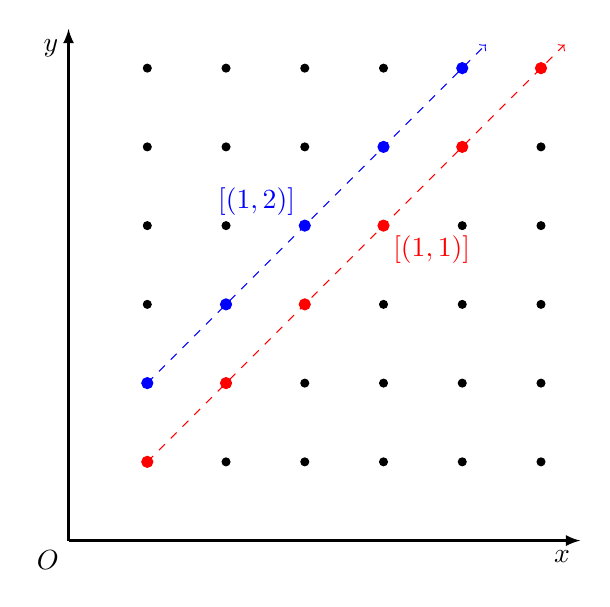
\begin{tikzpicture}[scale=1, transform shape]
            \draw[latex-, thick] (0, 6.5) node[below left]{$y$} -- (0, 0);
            \draw[latex-, thick] (6.5, 0) node[below left]{$x$} -- (0, 0);
            \node[below left] at (0, 0){$O$};
            \foreach \x in {1,...,6}{
                \foreach \y in {1,...,6} {
                    \draw[fill] (\x, \y) circle (0.05);
                }
            }

            \draw[color=red, dashed, ->] (1, 1) -- (6.3, 6.3);
            \node[below right, color=red] at (4, 4){$[(1, 1)]$};
            \foreach \x in {1,...,6} {
                \draw[fill, color=red] (\x, \x) circle (0.07);
            }

            \draw[color=blue, dashed, ->] (1, 2) -- (5.3, 6.3);
            \node[above left, color=blue] at (3, 4){$[(1, 2)]$};
            \foreach \x in {1,...,5} {
                \draw[fill, color=blue] (\x, \x + 1) circle (0.07);
            }
        \end{tikzpicture}
        \end{center}
    \end{enumerate}



    \paragraph{Problem 6.}
    \begin{enumerate}
        \item Let all $x_i \in \mathbb{R}\setminus\{0\}$ in the following discussion.

        Clearly, $\sim$ is reflexive since $(x_1, x_2) = 1\cdot (x_1, x_2)$.

        Let $(x_1, x_2)\sim(x_3, x_4)$. Then, $(x_3, x_4) = \alpha (x_1, x_2)$
        for some $\alpha \neq 0$, hence $(x_1, x_2) = \frac{1}{\alpha}(x_3,
        x_4)$. Therefore, $\sim$ is symmetric.

        Let $(x_1, x_2) \sim (x_3, x_4)$ and $(x_3, x_4) \sim \beta(x_5,
        x_6)$. Then, $(x_3, x_4) = \alpha(x_1, x_2)$ and $(x_5, x_6) =
        \beta(x_3, x_4)$ for some $\alpha, \beta \neq 0$. Thus, $(x_5, x_6) =
        (\alpha\beta)\cdot (x_1, x_2)$ and $\alpha\beta \neq 0$, so $(x_1,
        x_2) \sim (x_5, x_6)$.  Therefore, $\sim$ is transitive.

        Hence, $\sim$ is an equivalence relation.\qed

        \item For $(r, s) \in \mathbb{R}\setminus(0,0)$, its equivalence class
        is given by \begin{align*}
            [(r, s)]
                \;&=\; \{(x, y) \in \mathbb{R}^2\setminus\{(0, 0)\} : (r, s)\sim(x, y)\} \\
                \;&=\; \{(x, y) \in \mathbb{R}^2\setminus\{(0, 0)\} : (x, y) = \alpha(r, s), \alpha \neq 0\} \\
                \;&=\; \{(\alpha r, \alpha s) : \alpha \in \mathbb{R}\setminus\{0\}\}.
        \end{align*}
        Clearly, each equivalence class $[(r, s)]$ is a line of slope $s/r$,
        through $(1, s/r)$, excluding the origin in the Cartesian plane.

        \begin{center}
        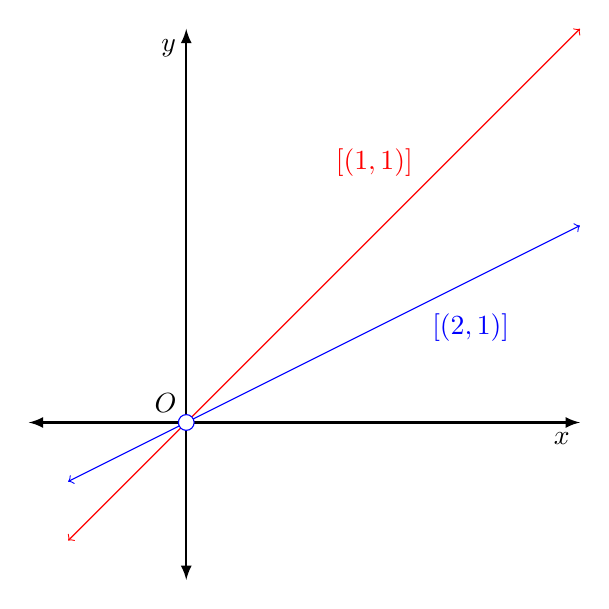
\begin{tikzpicture}[scale=1, transform shape]
                \draw[latex-latex, thick] (0, 5) node[below left]{$y$} -- (0, -2);
                \draw[latex-latex, thick] (5, 0) node[below left]{$x$} -- (-2, 0);
                \node[above left] at (0, 0){$O$};
                \node[above left, color=red] at (3, 3){$[(1, 1)]$};
                \draw[<->, color=red] (-1.5, -1.5) -- (5, 5);
                \node[below right, color=blue] at (3, 1.5){$[(2, 1)]$};
                \draw[<->, color=blue] (-1.5, -0.75) -- (5, 2.5);
                \draw[color=blue, fill=white] (0, 0) circle (0.1);
        \end{tikzpicture}
        \end{center}

    \end{enumerate}


    \paragraph{Problem 7.}
    \begin{enumerate}
        \item There are $2^{n^2}$ relations on $X$.

        This is because every relation on $X$ is simply a subset of the
        Cartesian product $X \times X$, and vice versa. This means that there
        are exactly as many relations on $X$ as there are subsets of $X \times
        X$. Now, there are $n^2$ elements of $X\times X$, hence $2^{n^2}$
        subsets of $X\times X$. \qed


        \item There are $2^{n^2 - n}$ reflexive relations on $X$.

        Denote $\Delta = \{(x, x) \colon x \in X\}$, the \emph{diagonal} of
        $X\times X$. Clearly, there are $n$ elements in $\Delta$.

        With this, note that a relation $R$ on $X$ is reflexive if and only if
        $\Delta \subseteq R$. This means that there are exactly as many
        reflexive relations on $X$ as there are subsets of $X\times X$ which
        contain $\Delta$. Of the $n^2$ elements of $X\times X$, we have $n$ of
        them in $\Delta$, leaving $n^2 - n$ elements free to either be or not
        to be in $R$. As a result, we have $2^{n^2 - n}$ such subsets of
        $X\times X$. \qed


        \item There are $2^{n(n + 1) / 2}$ symmetric relations on $X$.

        Enumerate $X = \{x_1, \dots, x_n\}$. Note that when forming a
        symmetric relation $R$ on $X$ by choosing a subset of $X\times X$,
        the choice of any $(x_i, x_j)$ where $i \leq j$ forces the choice of
        $(x_j, x_i)$. Furthermore, any symmetric relation on $X$ can be formed
        in this way. This means that there are exactly as many symmetric
        relations on $X$ are there are subsets of \[
            U = \{(x_i, x_j) \in X\times X\colon 1 \leq i \leq j \leq n\}.
        \] Clearly $U$ has $1 + 2 + \dots + n = n(n + 1) / 2$ elements, hence
        $2^{n(n + 1) / 2}$ subsets. \qed


        \item There are $2^{n(n - 1) / 2}$ reflexive and symmetric relations
        on $X$.

        Note that when forming a reflexive and
        symmetric relation $R$ on $X$ by choosing a subset of $X\times X$, the
        choice of all $(x_i, x_i)$ where $1 \leq i \leq n$ is forced (by
        reflexivity). Additionally, the choice of any $(x_i, x_j)$ where $i <
        j$ forces the choice of $(x_j, x_i)$. Finally, any reflexive and
        symmetric relation on $X$ can be formed in this way. This means that
        there are exactly as many symmetric relations on $X$ are there are
        subsets of \[
            U' = \{(x_i, x_j) \in X\times X\colon 1 \leq i < j \leq n\}.
        \] Clearly $U'$ has $0 + 1 + \dots + (n - 1) = n(n - 1) / 2$ elements,
        hence $2^{n(n - 1) / 2}$ subsets. \qed
    \end{enumerate}


\end{document}
